\section{Community Detection State of the Art}\label{C3}
\begin{figure}[h]
	\centering
	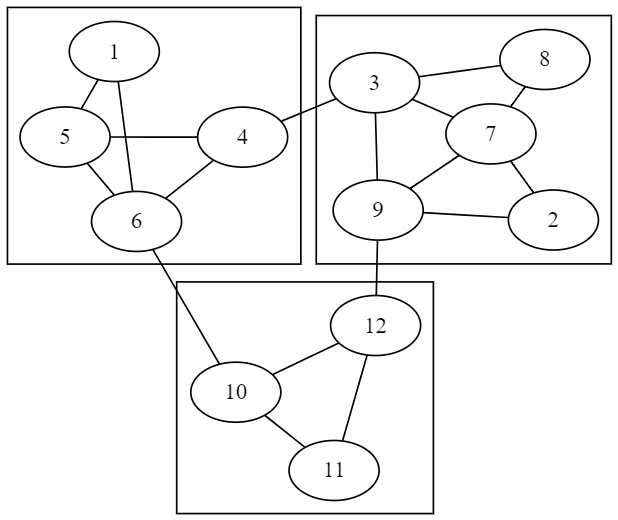
\includegraphics[width=0.6\linewidth]{0-resources/community1}
	\caption{An example of a communities structured graph. Three communities are enclosed by the rectangles.}
	\label{fig:community1}
\end{figure}
\noindent The problem of community detection raises in many application scenarios from the necessity of finding groups of objects that have a large number of connections to each other. To represent problems where it is fundamental to empathize connection between objects, the graph theory is the main tool. A graph is a mathematical structure composed of nodes (or vertices) that denote the objects and edges (or links) that express some kind of relationship between objects and possibly having a weights that quantifies this relationship.
The Graph Theory born in 1736 when Euler used this mathematical abstraction to solve the puzzle of Königsberg’s bridges. Since then, this tool was used in several of Mathematics, Social, Biological and Technological application. In recent time, the approach to this studies has been revolutionized to deal with bigger and more complicated challenges, supported by the increasing computing power.
\begin{figure}[h]
	\centering
	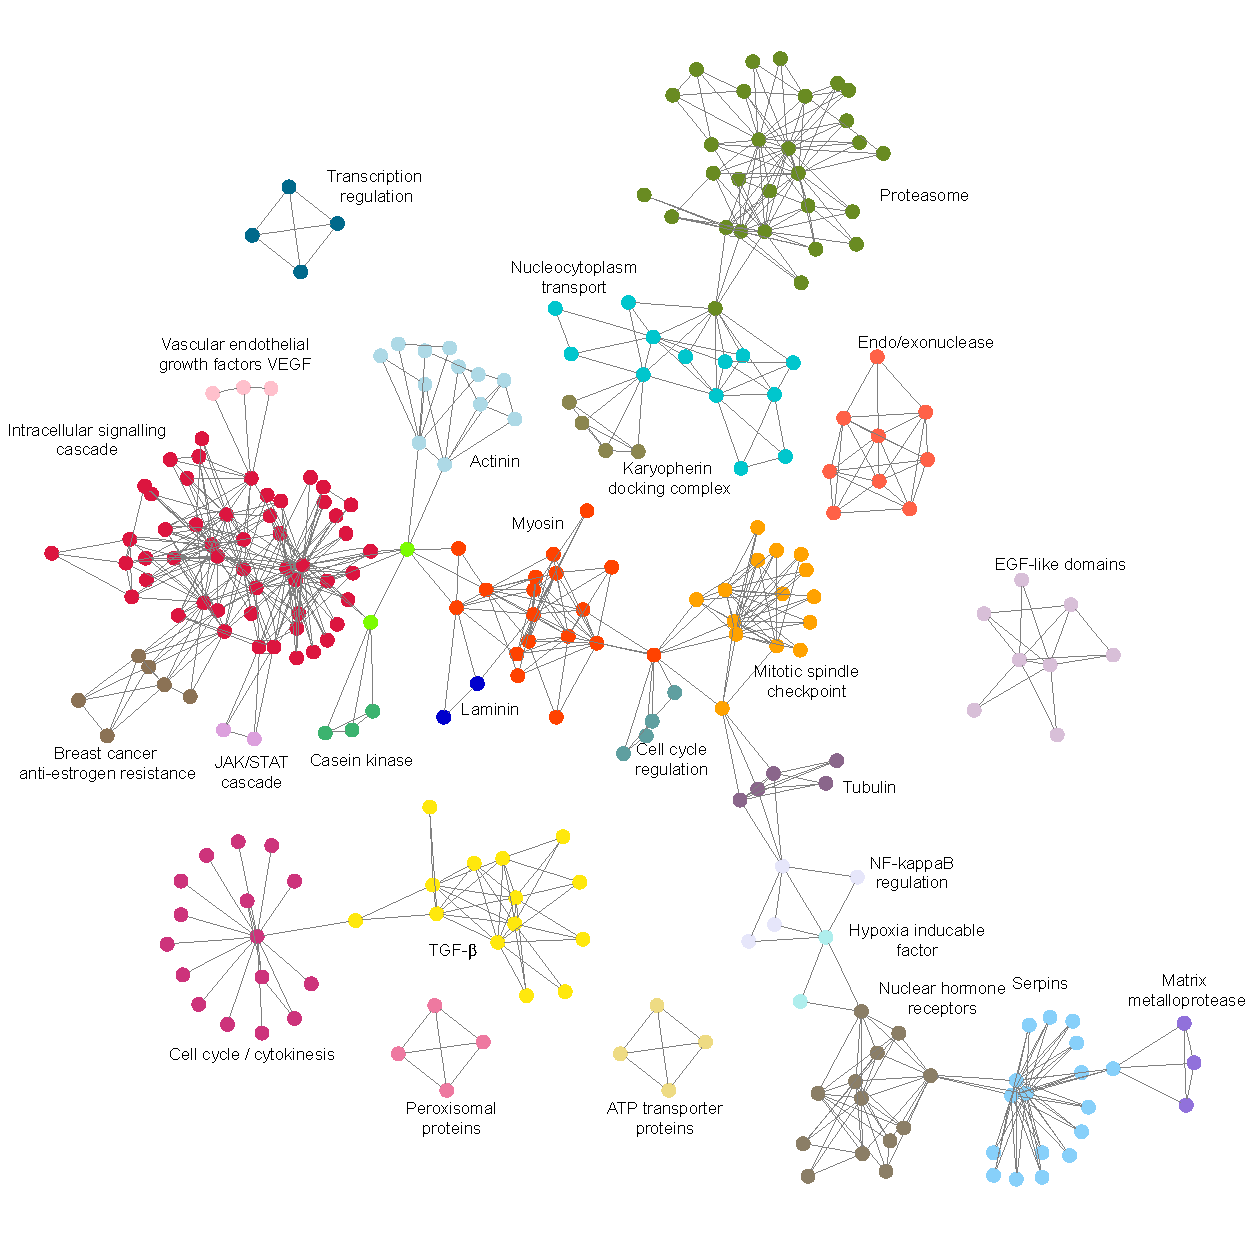
\includegraphics[width=1\linewidth]{0-resources/ppi}
	\caption{A protein protein iteration network of a rat cancerous cell. This image was reprinted from \cite{metastasis}.}
	\label{fig:ppi}
\end{figure}\\
The necessity of finding this high-connected substructure in graph arises from real problems in different research areas: for example, the study of Protein-Protein Interaction (PPI) networks is very important because the interaction between proteins is the basis of all process in the cell.\\ A study demonstrated that this type of network shown to be useful for highlighting key proteins involved in metastasis. \cite{metastasis} \\
Other examples can be found in the field of sociology: a historically well-know scenario is the Zachary's Karate Club. This dataset captures members of a Karate Club for 3 years.\cite{Zac77} An edge between two nodes represents an interaction between two members outside the club. At some point, a conflict between the administrator and a master led to split of the club into two separate groups. The question is if it is possible to infer who compose these two new groups basing on the information that this graph give to us. 
\begin{figure}
	\centering
	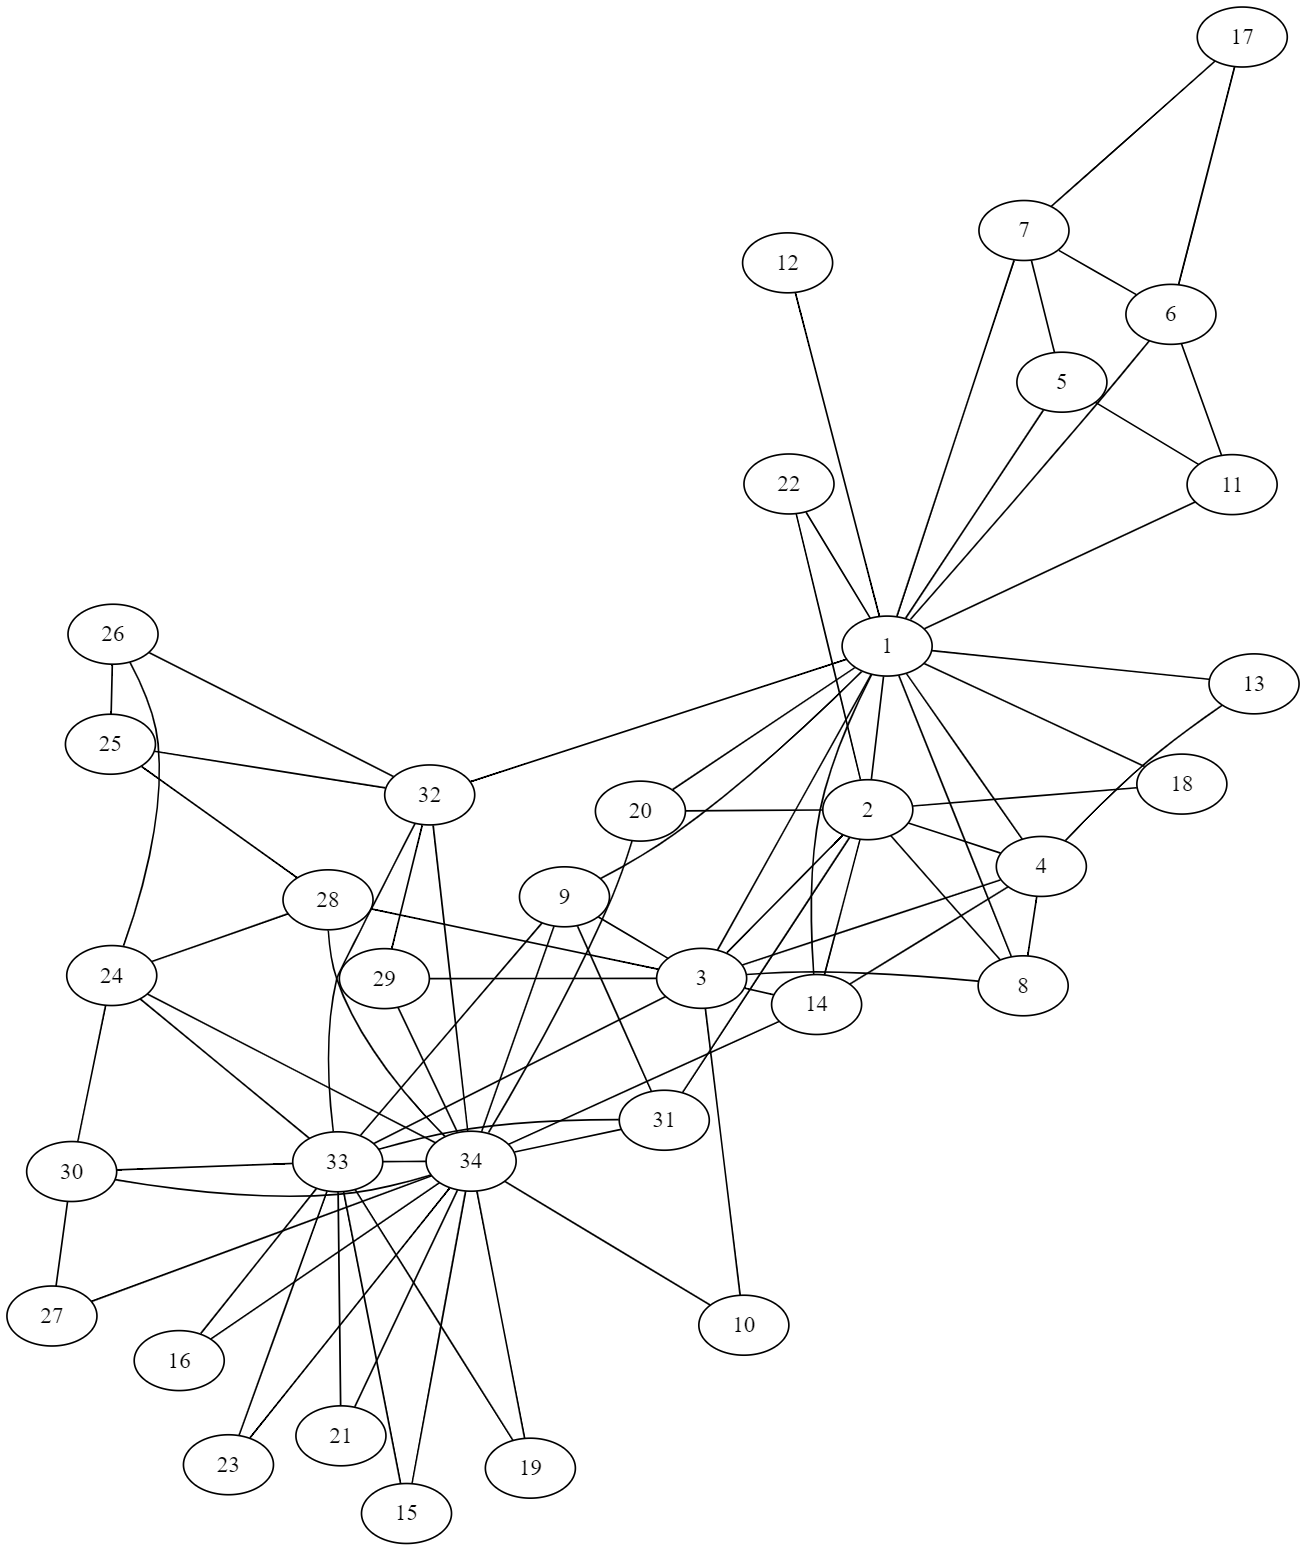
\includegraphics[width=0.6\linewidth]{0-resources/karateclub}
	\caption{Zacahry's karate club. \cite{Zac77} This image was made with Graphviz.}
	\label{fig:karateclub}
\end{figure}
This small network of 1977 is famous because it has often been used as a reference point to test the detection algorithms used to analyze huge social web networks.
In general this kind of problem, i.e. clustering people that belong to the same community base on interaction, it's useful not only in sociology but also in marketing: by knowing people with similar interests, it's possible to make better recommendation systems.\\
There are several of similar real-world scenarios, all united by the fact that the data is unregular but it's present some well-defined topological structure that in a completely random graph are absent. A random graph is a fully disordered graph, firstly proposed by Erdös and Rényi \cite{random} in 1959: it's a graph where the probability that there is an edge between two nodes it's equal for all pairs of nodes and, for this reason, the degree of the nodes (i.e. the number of edges incident to a node) is homogeneous. In real networks, this is not true, because they are often scale-free (follow a power-law distribution). An example of this is the study about the citations in scientific papers made by Derek J. de Solla Price in 1965 \cite{dsp} or the study about World Wide Web growing made by Albert-László Barabási et al in 1999 \cite{Barab}.
Furthermore, the degree distribution of the nodes is non-homogeneous not only globally but also locally, this due to the observation that there is a high concentration of edges within sets of nodes and a low concentration of edges between this sets. These two concepts are essential to formulate the formal definition of Community and Modularity. In this chapter will be presented some definitions of community and will be given an overview of some methods that are used to identify communities.
\subsection{Community Definitions}\label{3.1}
The informal definition of community is there are many more edges inside the community versus the rest of the graph, but there isn't a unique quantitative definition of community. This kind of freedom is necessary because the concept of community is strictly connected to the problem that will be analyzed: for example, in some cases, it's necessary that communities overlap, but in other problems, this is not necessary. There is a unique key constraint that allows talking about community detection: the graph must be sparse. A sparse graph is a graph where the number of nodes has the same magnitude of the number of edges. In the unweighted graph case, if the number of edges is far greater than the number of nodes, the distribution of edges among the nodes is too homogeneous for communities to make sense \cite{fortunato}. In that case, the problem nature is little different: we aren't interested anymore on the edge density between nodes but we have to use some kind of metrics (like similarity or distance) to clustering. In that case, the problem is more similar to data clustering. Despite this, assuming that a community is a subset of similar nodes it's reasonable, for this reasons some techniques (like spectral o hierarchical clustering) belonging to this field are adopted in community detection and will be shortly presented later on this thesis.
Following this, Fortunato \cite{fortunato} defines three main classes of community's definitions: \textit{local, global and based on vertex similarity}. Other types of definitions are still possible, but these three offers give a good summary of the problem. We now present those classes to give an overview of the various approach that has been used to define this problem. 
\subsubsection{Local definitions}\label{local-def}
Considering that a community has a lot of interactions with the other nodes that are in it and few connections outside, it is fair to think about the communities as autonomous objects.
The local definitions are based on this concept. Directly from this concept, we can think at the community as a clique, i.e. a subset whose vertices are all adjacent to each other. This type of definitions it's too strict: even if just one edge is not present, the subset is not a clique, but the subset has a very high concentration of edges. For this reason, the clique definition is often relaxed, using, for example, $n$-clique, i.e. a subset in which all the vertices are connected by a path of length less than $n$.\\
Anyway, this type of definitions ensure that there is a strong cohesion between the nodes in the subset, but it does not ensures that there isn't a comparable cohesion between the subset and the rest of the graph. For this purpose, other definitions were proposed. 
Given a graph $G(V,E)$, the corresponding adjacency matrix $A$ and a subset of nodes $C$ where $C \in V$, we define the internal degree $k_v^{int}$ and the external degree $k_v^{ext}$ for each vertex $v$ that belongs to $C$ as the number of edges that connect the node $v$ with another node that belongs to $C$ and not belongs to $C$, respectively:
\begin{align}
k_v^{int}= \sum_{k \in C} A_{vk} && k_v^{ext}= \sum_{k \notin C} A_{vk}
\end{align}
where $A_{vk}$ is the entry of $A$ at position $(v,k)$. We also define the internal degree $k_C^{int}$ and the external degree $k_C^{ext}$ as the sum of all internal and external degree of nodes that belongs to $C$. 
\begin{align}
k_C^{int}= \sum_{i,j \in C} A_{ij} && k_C^{ext}= \sum_{i\in C, j \notin C} A_{ij}
\end{align}
A strong community is a subset of nodes such that the internal degree $k_n^{int}$  for each vertex $n$ is greater than its external degree $k_n^{ext}$ . This type of definitions once again very strict, for this reason we define as weak community a subset of nodes where the internal degree of the subset  $k_C^{int}$ is greater than its external degree $k_C^{ext}$. Many other variants of these definitions were presented in the literature.
\subsubsection{Global definitions}
The previous class quantifies the communities independently, considering every subset individually. Overturning the point of view, we can define communities in a graph-dependent way, considering them as an essential and discriminant part of it. There are many different interpretations of this approach in the literature, but the most important definitions are focused on this key fact: it's not expected to see a community structure in a random graph. For this reason, we define as \textit{null model} of a graph another graph that has some features in common with the original one but it's generated randomly. This graph is used as a comparison term to identify if it's present a community structure in the graph or not and, if it is present, to quantify how it is pronounced.
The comparison between a graph and the corresponding null model, which is based the Modularity Optimization, is the main object of this study and is presented in detail in the next chapter.
\subsubsection{Based on Vertex Similarity}
The last class of definitions assumes that edges in the same community are similar to one another. All the definition used in the classic clustering methods belongs to this class because they calculate a distance (similarity) between object and aren't based on the edge density like the previous definitions. This distance can be calculated in various ways:  if it is possible to embed the vertices into a $n$-dimensional Euclidean space by assigning a position to them, one method consists to calculate the distance between two nodes, considering that similar vertices are expected to be close to each other. To calculate the distance, one could use a norm. Three norms often used in the literature are the following. Given two points $a=(a_1, ... , a_n)$ and $b=(b_1, ... , b_n)$ that belongs to the $n$-dimensional Euclidean space $E$, we define the norms $l_1$ (Manhattan distance), $l_2$ (Euclidian distance) and $l_3$ (Maximum distance) as:
\begin{align}
l_1(a,b) =&\sum_{k=1}^{n} |a_k - b_k|\\
l_2(a,b) =&\sum_{k=1}^{n} \sqrt{(a_k -b_k)^2}\\
l_3(a,b) =&\max_{k \in [1,2]} |a_k - b_k|
\end{align}
Another option is the cosine similarity $\cos(a, b)$, that is very popular in literature:
\begin{equation}
\cos (a,b) = \frac{ \sum_{i=1}^{n}{{a}_i{b}_i} }{ \sqrt{\sum_{i=1}^{n}{({a}_i)^2}} \sqrt{\sum_{i=1}^{n}{({b}_i)^2}} }
\end{equation}
If it is not possible to embed the graph in a Euclidean Space, it is possible to infer the distance from the adjacency matrix. 
If it is not possible to embed the graph in a Euclidean Space, it is possible to infer the distance from the adjacency matrix. One idea is to map the distance in order to assign smaller values at nodes with the same neighbourhood. Given an adjacency matrix $A$ we define the distance between two nodes $a$ and $b$ as:
\begin{equation}
d(a,b) = \sqrt{\sum_{k\ne a,b} (A_{ak} - A_{bk})^2} 
\end{equation}
Many other variants of that definition (but based on the same principle) were presented in the literature, for example considering the overlap between neighbourhood respect to the union. \\
Other alternative measures consider the number of independent paths between nodes, i.e. path that does not share any common edges, or they are based on random walk on a graph: for example, the average number of steps needed to reach one vertex from another by a random walker.  

\subsection{Community Detection Algorithms}
A partition is a division of the graph in clusters, such that each vertex belongs to exactly one cluster. 
The partition of possible partitions of a graph $G$ with $n$ vertices grows faster than exponentially with $n$,  thus making it impossible to evaluate all the partitions of a graph \cite{fortunato}. For these reasons, many techniques were introduced to find the most significant ones.
We now present an introduction to some classical class of techniques used in the field of community detection: Partitional clustering, Graph partitioning, Spectral clustering, Hierarchical clustering.  Moreover, the Girvan and Newman algorithm is presented later on: even if this method is a Hierarchical algorithm, this method firstly introduced the modularity function and it is presented separately. The goal of this chapter is to give a useful overview in order to get the differences with the Modularity optimization and empathize the motivations that led to the choice of the Louvain algorithm, one of the most used nowadays, especially for huge graphs. For this reason, all the methods that are presented in this thesis find a partition, as the Louvain methods. 
For the sake of completeness, we remark that in Fortunato's report \cite{fortunato}, that was mainly used to write this chapter, is presented an analysis of algorithms that found also overlapping communities (covers). 
\subsubsection{Partitional clustering}
Partitional clustering is a class of methods that find clusters from data points. The algorithms in this class embed the graph in a metric space as seen in chapter \ref{local-def}, and then calculate the distance between these new points.  The goal is to separate the points in $k$ clusters minimizing the distance between points and to the assigned centroids (i.e. the arithmetic mean position of all the points in the cluster). The number of clusters $k$ is given as input. The most famous technique is k-means clustering.
The objective function to minimize is the following:
\begin{equation}
\sum^k_{i=1} \sum_{x_j\in C_i} || x_j - c_i ||^2 
\end{equation}
where $C_i$ is the $i$-th cluster and $c_i$ is its centroid. This function quantifies the intracluster distance. 
At the start, the $k$ centroids are set far distance from each other. Then, each vertex is assigned to cluster with the nearest centroid and the centroid is recalculated.  Even if the method doesn't find an optimal solution and the solution is strongly dependent on the initial setup of the centroids, this method remains popular due to the quick convergence that allows it to analyze big graphs.
However, setting the apriori number of cluster $k$ is not simple to estimate that number,
especially in a large graph, and for this reason, it is often preferred algorithms that can automatically derive it. Moreover, the embedding of the graph in the Euclidean Space may be tricky and not reliable for some graphs.
\subsubsection{Graph partitioning} 
Given a graph $G(V, E)$ and a number $g$ of clusters, the problem of graph partitioning consists of creating a partition of nodes composed by $g$ subsets such that it minimizes the edges lying between the clusters. To archive this goal, many algorithms perform a bisection of the graph, even for partitions with more than two clusters, where the bisection is iterated.  One of the earliest and famous algorithms is the Kernighan–Lin algorithm. This algorithm performs an optimization of the function $Q = link_{in} - link_{between}$, where $ link_{in}$ is the number of edges inside the subsets and $link_{between}$ is the number of edges lying between them. The algorithm starts from an initial partition (randomized or suggested by the graph), and the algorithm performs a swapping between clusters for a fixed number of nodes pair to increase the value of $Q$. 
To avoid local maxima, some swaps that decrease $Q$ are kept. 
With some optimizations, the complexity of this algorithm is $O(n^2)$ where $n$ is the number of nodes.\\
Other techniques are based on the max-flow min-cut theorem by Ford and Fulkerson \cite{ford} and the minimization of cut-affine measures, like the normalize cut:
\begin{equation}
\Phi_N(C) = \frac{c(C, V/C)}{k_c}
\end{equation}
where $C$ is a subset of nodes, $k_c$ is the total degree of $C$ and $c(C, V/C)$ is the sum of all the edges lying between the subsets $C$ and $V/C$. \\
Like the previous class, specifying the number of clusters is the greatest limit of this class of algorithm. In additions, iterative bisecting can lead to not reliable clusters, because the sub-clusters are made breaking the previous ones:  in this way, the new subsets have vertices only from one of the "parent" cluster.  
\subsubsection{Spectral clustering}
Given a set of $n$ object $x_1 ,x_2, ..., x_n$ and the matrix $S$ of pairwise similarity function $s(x_1, x_2)$ such that $s$ is symmetric and non negative, we define as spectral clustering all methods that using the eigenvector derived from the matrix $S$ to cluster the data.
In particular, this transformation makes a change from the reference system of the object to another whose coordinates are elements of eigenvectors. This transformation is made to enhance the proprieties of the initial data.  After that, we can cluster the data using other techniques as $k$-means and obtain a better result. The Laplacian matrix is the most used in spectral clustering. Given a graph $G$ and its associated adjacently matrix $A$, we define the Laplacian matrix $L$ of the graph $G$ as:
\begin{equation}
L = D - A 
\end{equation}
where $D$ is the degree matrix, a diagonal matrix which contains information about the degree of each vertex. This matrix is used due to nice propriety: if the graph has $k$ connected components, the Laplacian of the graph will have $k$ zero eigenvalues.
In that case, the matrix can be organized in a way that displays $l$ square blocks along
the diagonal. When is it in this block-diagonal form, each block is at his turn a Laplacian matrix of one of the subcomponent.
In this situation,
there are $k$ degenerate eigenvectors with equal non-vanishing components in correspondence with the vertices of a block and zero otherwise. 
Considering the $n\times k$ matrix where $n$ is the number of nodes of $G$ and the columns of this matrix are the $k$ eigenvectors, we can see that vertices in the same connected component of the graph coincide.
If the graph is connected but the connections between the $k$ subgraph are weak, only one eigenvalue is zero. By the way, However, the lowest $k - 1$ non-vanishing eigenvalues are still close to zero and the vertex vector of the first $k$ eigenvectors still identify the clusters.\\
An application of these techniques is the spectral bisection methods: this algorithm combines ideas from spectral clustering and graph partitioning. 
Given the graph $G$ with $n$ nodes, the cut size $R$ of the bipartition of the graph is:
\begin{equation}\label{spec_bi_pa}
R = \frac{1}{4} s^TLs
\end{equation} 
where $L$ is the Laplacian matrix and $s$ is the $n$-vector that represents the affiliation of the nodes to a group (if the node $i$ belongs to the first group, the $i$-th entry of $s$ will be $1$, $-1$ otherwise).
$s$ can be writtens as $s= \sum_{i=0}^n a_i v_i$ where $v_i$ is the $i$-th eigenvector of the Laplacian.
If $s$ is normalized, we can write the equation (\ref{spec_bi_pa}) as follows:
\begin{equation}\label{spec_bi_pa}
R = \sum_{i=0}^n a_i^2 \lambda_i
\end{equation} 
where $\lambda_i$ is the eigenvalue corresponding to $v_i$.
From this, choosing the $s$ parallel to the second-lowest eigenvector $\lambda_2$ we have a good approximation of the minimum because this would reduce the sum to $\lambda_2$. We remark that we use the second one because the first one is equal to zero. To cluster the data in the vector $s$, we match the signs of the components of $v$. \\
The exact computation of the all eigenvalues requires time $O(n^3)$, a too high complexity for big graphs, but there exist some techniques that allow calculating approximate values faster \cite{fortunato}.
 
\subsubsection{Hierarchical clustering}
The possible partitions of a graph can be very different in scale and some cluster in turn may show an internal community structure. In that case, there is a hierarchy between partitions. The most common way to represent this kind of structure is to draw a dendrogram, i.e. a diagram representing a hierarchical tree. If we draw an horizontal line in the dendrogram, observations that are joined together below the line are in the same cluster (Figure \ref{fig:dend}). The hierarchical clustering algorithms build an entire dendrogram starting or from the bottom (agglomerative algorithms), or from the top (divisive algorithms) using a similarity function to cluster. In the first type of algorithms, each node is initially considered as an independent community and the clusters are iteratively merged if the similarity score exceeds a threshold. A divisive algorithm inverts the starting point: at the start, all nodes belong to one single community and then the clusters are iteratively split. An example of this type of algorithm, the Girvan and Newman algorithm, is presented later on this thesis. 
\begin{figure}
	\centering
	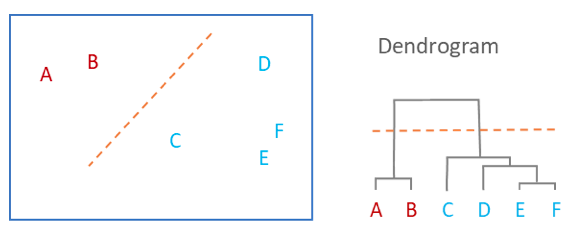
\includegraphics[width=0.7\linewidth]{0-resources/dend.png}
	\caption{Example of dendrogram. At left we have the data in a Euclidean space, at right we have the dendrogram. The dotted line in the dendrogram divides the data in two cluster, and we show the corresponding line in the Euclidean space. }
	\label{fig:dend}
\end{figure}
The algorithms that belong to this class doesn't need the number 
of clusters as input, but there is the problem of discriminating between the obtained partitions: with these algorithm we obtain a entire hierarchies of partitions (from the partition in which each nodes is in a different communities to the one with all the nodes are in a unique community) and we haven't a directed way to isolate the best ones. We need some quality function to find the best partition and the Modularity Function was introduced to overcome this problem. Moreover, as we see in the Girvan and Newman algorithm, building the entire hierarchy using similarity metrics requires a lot of computations: for these reasons the complexity of this class of algorithms tends to become much heavier if the calculation of the chosen similarity measure is costly \cite{fortunato}.

\subsection{Modularity Optimization}
Historically, the modularity function $Q$ was introduced as a stop criterion for the Girvan and Newman algorithm in 2002. It is a quality function, i.e. a function that allows distinguishing from a "good" clustering and a "bad" one. The function assigns to a partition a score that is used to compare partitions. This is not a trivial goal, because defining if a partition is better than another is an ill-posed question: the answer may depend on the particular concept of community that it is adopted. Nevertheless, this sometimes is necessary, for example in the case of hierarchical clustering, where it's necessary to identify the best partition in the hierarchies. A simple example is the sum of the difference between internal degree $k_v^{int}$ and the external degree $k_v^{ext}$ [\ref{local-def}]. \\
The modularity function became very popular and a lot of methods based on this quality function were created.
In this chapter we present the functions and their limits in details, the algorithm in which it was firstly used and some optimization techniques based on modularity.
\subsubsection{Modularity}
The function is based on the idea that a random graph would not exhibit a community structure.
We define as \textit{null-model} of a given graph, another graph that is generated randomly yet keeping some structural proprieties of the original one.
Comparing the graph with its null model, we can quantify how much the community structure is well defined. Therefore, the modularity function is dependent on the choice of the null model. 
Given an undirected graph $G = (V,E)$, a partition of nodes $C$ and a function $c(x)$ that assign each node $x$ to its community, we define a generic modularity function as :
\begin{equation}\label{Q1}
Q = \frac{1}{2|E|} \sum_{i,j \in V}(A_{ij} - P_{ij}) \delta(c(i), c(j))
\end{equation}
where $A$ is the  adjacency matrix of $G$, $P$ is the matrix of expected number of edges between nodes in the null model and $\delta$ is an filter function: its yields one if $c(i) = c(j)$, zero otherwise.\\
In principle, the choice of a null model is arbitrary, but we have to consider carefully the graph properties to keep in the null model because they determine if the comparison is fair or not. 
For instance, it's possible to choose as a model that keeps only the nodes and edges numbers, assuming that an edge is present with the same probability for each pair of nodes (in this case $P_{ij}$ is constant). 
For this reason, The standard null model of modularity imposes that the expected degree sequence(after averaging over all possible configurations of the model) matches the actual degree sequence of the graph \cite{fortunato}.
In this scenario, the probability that two vertices $i$ and $j$ are connected by an edge is equals to the probability to get two stubs (i.e. half-edges) incident to $i$ and $j$.\\
This probability $p_i$ of piking a stub from the nodes $i$ is $\frac{k_i}{2|E|}$ where $k_i$ is the degree of nodes $i$. The probability that two stub joining is $p_ip_j = \frac{k_ik_j}{4|E|^2}$. Therefore, the expected number $P_{ij}$ of connections between the nodes $i$ and $j$ is:
\begin{equation}\label{Pij}
P_{ij} = 2mp_ip_j = \frac{k_ik_j}{2|E|}
\end{equation}
Replacing $P_{ij}$ from (\ref{Pij}) in (\ref{Q1}) we obtain:
\begin{equation}\label{ModularityExt}
Q = \frac{1}{2|E|} \sum_{i,j \in V}\left(A_{ij} - \frac{k_ik_j}{2|E|}\right) \delta(c(i), c(j))
\end{equation}
that is the standard modularity function. This function can be rewritten considering that only the vertex pairs in the same community contribute in the sum: 
\begin{equation}\label{ModularityC}
Q =  \sum_{c}^{|C|} \left( \frac{l_c}{|E|} - \left( \frac{k_c}{2|E|}\right) ^2 \right)
\end{equation}
where $l_c$ is the sum of edges that connect nodes in $c$ and $k_c$ is the sum of degree of nodes that belongs to $c$, i.e. total degree. \\
The modularity function $Q$ it is in range [-1/2, 1] \cite{bounds}, and if we consider the whole graph as a unique community $c$ we obtain $Q = 0$. Opposite, if we consider each nodes as community, $Q < 0$. Then, if a partition has a modularity score $<0$, the partition hasn't a modularity structure. 
\subsubsection{Resolution Limit}
There is a well-known limit of the modularity function, identified by Fortunato and Barthélemy \cite{resolution-limit} in 2006. Considering (\ref{Pij}), we can easily compute the expected number of edges $P_{AB}$ between two clusters $c_A$ and $c_B$, that are separate cluster in partitions $C$, as:
\begin{equation}
P_{AB} = k_A k_B /2m 
\end{equation}
where $k_a$ ($k_a$) is the total degree of $c_a$ ($c_b$).
We can compute from (\ref{ModularityC}) the difference $\Delta Q_{AB}$ that affecting the modularity when we consider $c_A$ and $c_B$ in a partition where they are two different cluster, with respect to the partition where they are merged in one cluster $c_{AB}$:
\begin{equation}\label{DQAB}
\Delta Q_{AB} = \frac{l_{AB}}{|E|}  - \frac{k_Ak_B}{2|E|}
\end{equation}
where $l_{AB}$ is the sum of edges that connect nodes that belongs to $A$ to nodes that belongs to $B$.
Now considering the case $l_{AB} = 1$: there is only one edge that connects these two clusters. Therefore we expect that we obtain a greater modularity score keeping these two clusters separate with respect to merging them. Instead, from (\ref{DQAB}) we have that the modularity increase if  $\frac{k_Ak_B}{2|E|} < 1$. For the sake of simplicity, we assume that $k_A = k_B = k$. We obtain that if $k < \sqrt{2|E|}$, the modularity is greater if we merge the communities. From this it follows that if the communities are sufficiently small in degree, the expected number is smaller than one: in this case if there is only one edge between the two communities, we obtain a better result merging them. The result of this observation is that the modularity optimization has a resolution limit that prevents it to detect communities that are too small with respect to the graph as a whole.
This problem has many implications: the real networks have a community structure composed by communities very different in size, so some of these communities may be wrongly merged. Fortunato identifies as week point the assumption that in the null model each vertex can interact with every other vertex \cite{fortunato}. Some solutions are proposed, as tunable parameters that allow avoiding the problem or also algorithm that eliminate artificial mergers. Nevertheless, in many real cases, the modularity-based algorithms still obtain very good results and permit to analyze quickly very large graphs. For those reasons, the algorithms of this class remain the most used, but it's important to remark their limits.

\subsection{Girvan and Newman algorithm}
Now we present the Girvan and Newman algorithm \cite{Girvan2002Community}. This method deserves to be presented because it is the first method that uses the modularity as quality function \cite{Newman_2004} and it represents a turning point in the history of community detection. This method is a divisive algorithm, i.e. it tries to identify edges that connect two communities and then remove that edge. The goal of the algorithm is to get clusters disconnected from each other.  
To select which edge we have to remove, we introduce the concept of edge betweenness.
The edge betweenness it is a measure that quantifies how an edge is least central for a community. 
If an edge connected two communities, it should have a greater value compared to an edge that is incident to two nodes that are in the same community. \\
The algorithm has 2 steps iterated until all edges are removed:
\begin{enumerate}
	\item computation of the edge betweenness for each edge;
	\item removal of the edge with the largest betweenness (Figure \ref{fig:edgebtw});
\end{enumerate}
The algorithm constructs an entire dendrogram of partitions, and the modularity is used to select the best one.
\begin{figure}
	\centering
	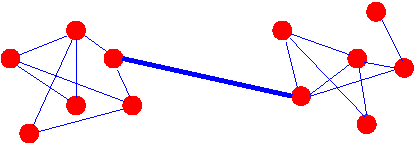
\includegraphics[width=0.7\linewidth]{0-resources/edgebtw}
	\caption{Considering the shortest path definition of the edge betweenness, the highlighted has the much higher values of betweenness than all other edges: indeed all shortest path connecting left vertices and right vertices run through it. For this reason, we chose to remove this edge and we obtain two clusters. This image was reprinted from \cite{fortunato2007community}. }
	\label{fig:edgebtw}
\end{figure}
\noindent Girvan and Newman proposed three different definitions of edges betweenness \cite{Newman_2004}: shortest-path, current-flow and random walk. The first one is the number of shortest paths between all vertices that include the edge (Figure \ref{fig:edgebtw}). The computation of this value for each edge of the graph has a complexity $O(n^2)$ on a sparse graph \cite{Newman_2004}. 
The second definition considers the graph as a resistor network created by placing a unit resistance on every edge of the network.
If a voltage difference is applied between any two vertices, each edge carries some amount of current.
The current flows in the network are governed by Kirchhoff’s equations and the calculations are performed on each edge in the graph.
This calculation has a complexity $O(n^3)$ on a sparse graph \cite{Newman_2004}. 
The last one is the expected frequency of the passage of a random walker on the edges. The calculation requires the inversion of the adjacency matrix followed by the calculus of the averaging flows for all pairs of nodes. The complexity is $O(n^3)$ on a sparse graph \cite{Newman_2004}. 
The first definition is the most used for its speed ($O(n^2) < O(n^3)$ and it is also shown that in practical application this edge betweenness gives better results \cite{Newman_2004}. The authors also show that the recalculation step is essential to detect correctly communities: this means that we have to recalculate the betweenness every time an edge will be removed, raising the complexity of the algorithm to $O(n^3)$ on a sparse graph. The complexity is the strongest limit of this algorithm, which, however, was the first one to introduce the modularity and has many ideas that were used later on.
\subsection{Modularity Optimization Techniques}
After the introduction of the modularity function $Q$, many algorithm were presented in the literature to directly optimize the modularity function $Q$. In this chapter we present the Newman's greedy algorithm which was the first one, in order to make a comparison with the Louvain algorithm that is also greedy. This algorithm also introduces for the first time the concept of $\Delta Q$, that will be expanded and used in the Louvain method. Moreover, we present also some other class of techniques that are used in modularity optimization like extremal optimization, simulated annealing and spectral clustering.
\subsubsection{Greedy Method of Newman}
\begin{figure}[h]
	\centering
	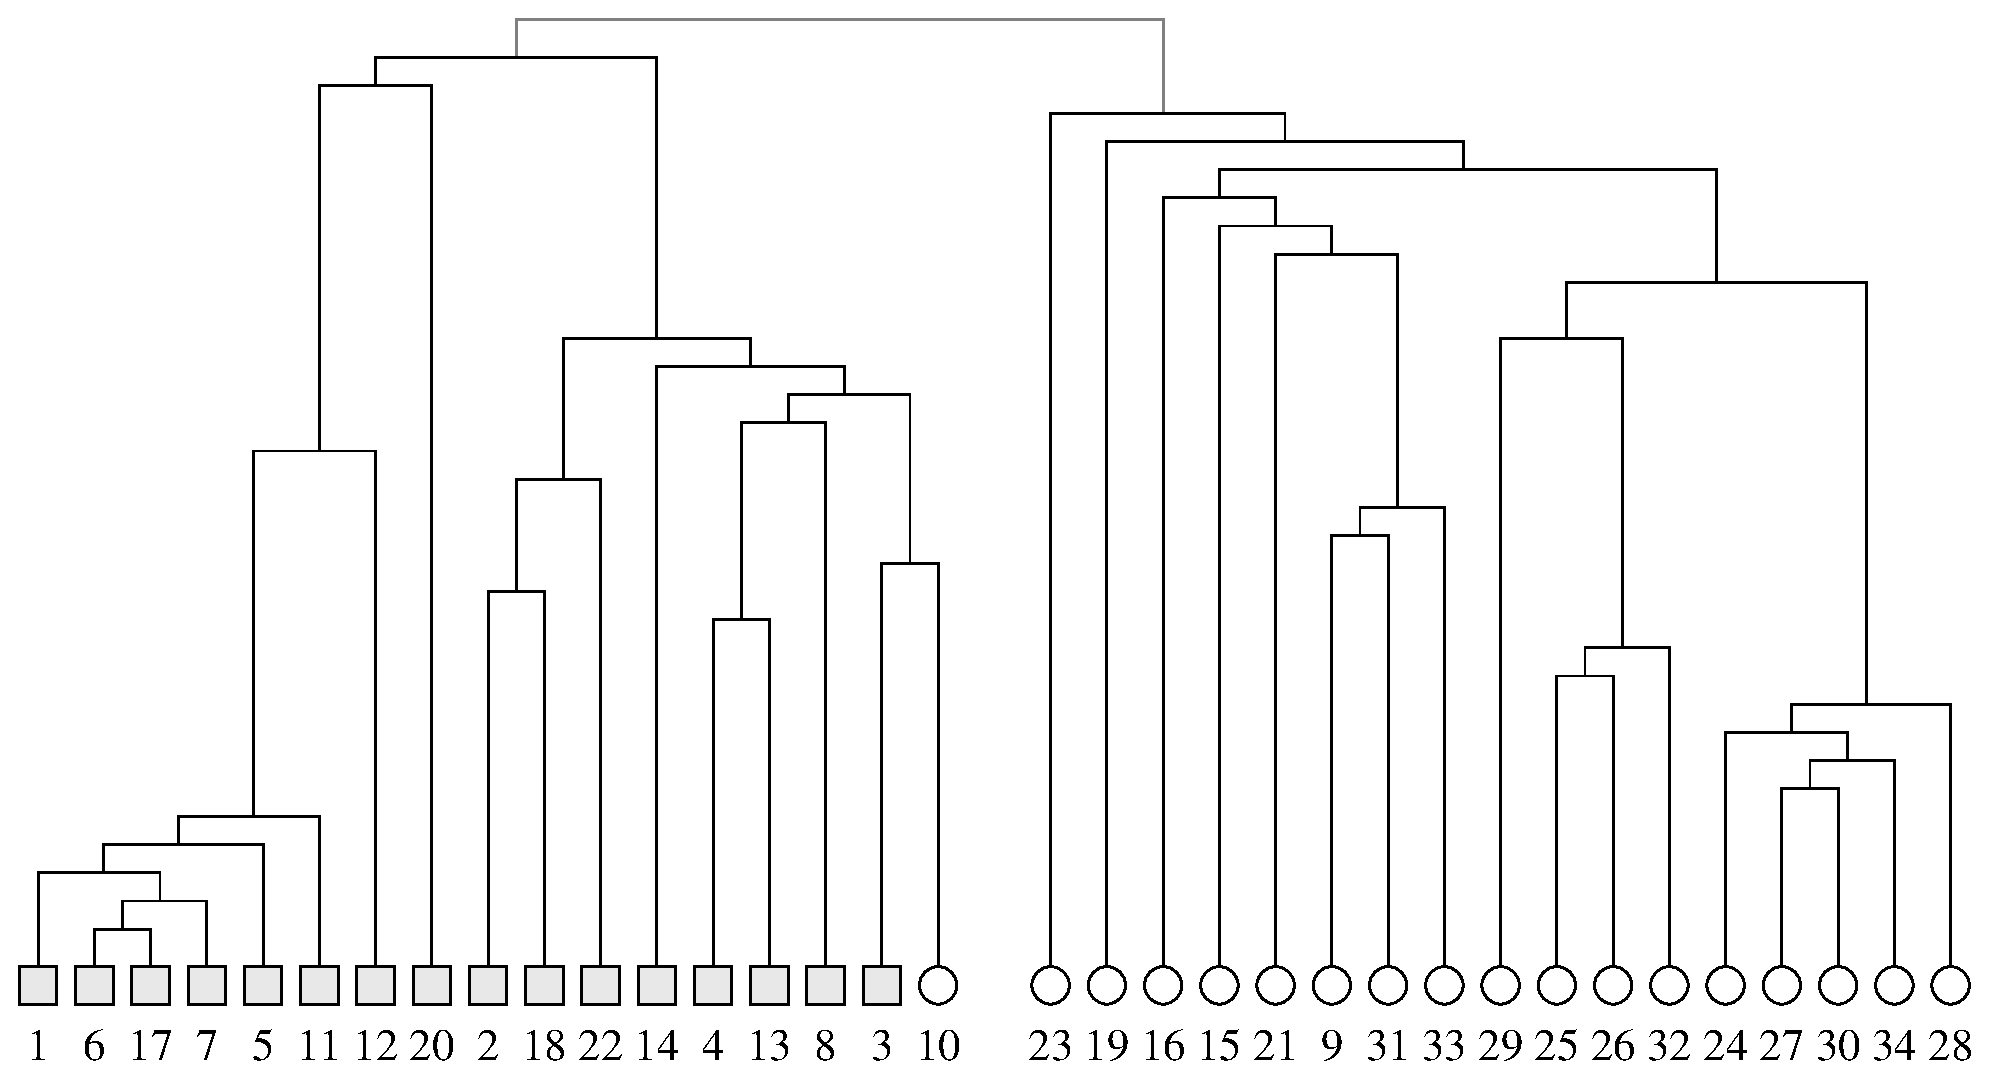
\includegraphics[width=0.7\linewidth]{0-resources/zachary}
	\caption{Dendrogram of the communities found by Newman algorithm in Zachary karate club network. This image is reprinted from \cite{Newman_greedy}.}
	\label{fig:dedro_zachary}
\end{figure}
The first modularity optimization algorithm is presented by Newman \cite{Newman_greedy},
and it is an agglomerative method. Given a graph $G(V,E)$ where $n$ are the number of nodes and $m$ the number of edges, the algorithm starts creating a supporting graph that represent the community structure. In this graph at the beginning there are all nodes and no edges between them: this represent the situation in which each node is assigned to a single cluster. The first step of the algorithm is to pick an edge from the original graph to add to the support graph such that it give the maximum increase (or minimal decrease) of the modularity with respect to the actual configuration. This value is indicated as $\Delta Q = Q_{now} - Q_{old}$ The modularity will be calculated on the full graph and not only on the "cluster" graph. Then we add the edge to the support graph: if the edges connect two sets of unconnected edges, it delivers a new partition and reducing by one the number of the partitions. So, the algorithm find $n$ different partitions of the graph (Figure \ref{fig:dedro_zachary}). 
We make some consideration of this procedure:
\begin{itemize}
\item If we add some edges that don't merge any partitions (i.e. it is internal), the modularity doesn't change.
\item Considering this, we have to calculate the modularity difference $\Delta Q$ only when we merge different partitions and so this operation is executed $n$ times.
\item Computing $Q$ requires a time of $O(m)$ that became $O(n)$ on a sparse graph.
\end{itemize}
For those reasons, the complexity of this algorithm is $O(n^2)$ on a sparse graph.
Many improvements of this algorithm were proposed later (like the Clauset et. al version \cite{Clauset_2004} that uses a max-heap to reduce the complexity to $O(n \log_2(n))$) but the complexity of the algorithm remains the biggest limit of it, even if this algorithm still allows to analyze large graphs.
\subsection{Other techniques}
The previous and Louvain algorithms are the two most famous greedy algorithms of community optimization, but other optimization strategies were proposed in the literature. A class of techniques are based on the concept of simulated annealing, i.e. an exploration of the space of the possible configuration looking for the maximum $Q$. 
Transitions between states are performed combining two types of "move": the first one assigns a vertex to a cluster chosen randomly; the second one merges or splits communities \cite{Guimer__2005}. These methods reach a very high score of modularity, near to the maximum. Unfortunately, it's very slow \cite{fortunato}. \\
To overcome this time problem, a heuristic denominated extremal optimization (EO) was proposed to perform an exploration of the space quickly. We define as fitness function $F$ of the vertex $x$ is the local modularity of $x$ divided by its degree. Starting from a random equal size bi-partitions of nodes, at each iteration a node is picked with a probability proportional to the score of the fitness measure and it is assigned to the other cluster. When there is no more improvement in modularity, the algorithm is called recursively on the two clusters. With a total complexity of $O(n^2 \log(n))$, this algorithm is a good trade-off between accuracy and speed \cite{eo}.\\ Finally, in literature it was presented the idea of combining modularity optimization with the spectral clustering. Given the adjacency matrix $A$ of the graph $G$, we define the matrix $B$ whose elements are:
\begin{equation}
B_{ij} = A_{ij} - \frac{k_ik_j}{2|V|}
\end{equation}
Modularity can be optimized by using spectral bisection on the matrix $B$ \cite{fortunato}. This algorithm has a total complexity of $O(n^2 \log(n))$.